% !TeX root = ../main.tex
\addcontentsline{toc}{section}{Introduction}
\section*{Introduction}
Ce chapitre détaille la réalisation technique du projet. Nous présentons l'environnement de développement, les technologies utilisées, l'intégration des modèles IA, le système d'agents, le traitement des documents, la génération des informations métier, le moteur de recherche, les API et les captures d'écran de l'application.

\section{Environnement de développement}
Le développement s'est déroulé sur un poste de travail équipé de Windows 11. L'environnement comprend Visual Studio Code comme IDE, Git pour la gestion de versions, Python 3.11 dans un environnement virtuel \texttt{.venv}, Docker Desktop pour la conteneurisation, Neo4j Community Edition en local et Ollama pour l'exécution locale des modèles de langage.

\section{Technologies utilisées}
Le tableau \ref{tab:stack} résume les technologies principales du projet.

\begin{table}[H]
    \centering
    \renewcommand{\arraystretch}{1.2}
    \begin{tabular}{|l|p{10cm}|}
        \hline
        \rowcolor{iNavy} \textbf{\color{white}Composant} & \textbf{\color{white}Rôle} \\ \hline
        LangGraph & Orchestration agentique sous forme de graphe d'état \\ \hline
        FastAPI & API REST et streaming Server-Sent Events \\ \hline
        Neo4j & Base de données graphe et index vectoriel \\ \hline
        Ollama & Exécution locale des LLM et modèles d'embedding \\ \hline
        Pydantic & Validation des schémas structurés \\ \hline
        pytest & Tests unitaires et d'intégration \\ \hline
        Docker Compose & Conteneurisation de l'API et des services \\ \hline
        Jinja2 / WeasyPrint & Génération de rapports PDF/HTML \\ \hline
        Streamlit & Interface utilisateur chatbot \\ \hline
    \end{tabular}
    \caption{Stack technique du projet}
    \label{tab:stack}
\end{table}

Les figures \ref{fig:tools_langgraph} à \ref{fig:tools_zammad} présentent les logos des principales technologies utilisées.

\begin{figure}[H]
    \centering
    \begin{minipage}{0.3\textwidth}
        \centering
        
\includegraphics[width=0.8\linewidth]{images/tools/langgraph.png}
        \caption{LangGraph}
        \label{fig:tools_langgraph}
    \end{minipage}%
    \begin{minipage}{0.3\textwidth}
        \centering
        
\includegraphics[width=0.8\linewidth]{images/tools/FastAPI.png}
        \caption{FastAPI}
        \label{fig:tools_fastapi}
    \end{minipage}%
    \begin{minipage}{0.3\textwidth}
        \centering
        
\includegraphics[width=0.8\linewidth]{images/tools/Neo4j.png}
        \caption{Neo4j}
        \label{fig:tools_neo4j}
    \end{minipage}
\end{figure}

\begin{figure}[H]
    \centering
    \begin{minipage}{0.3\textwidth}
        \centering
        
\includegraphics[width=0.8\linewidth]{images/tools/ollama.png}
        \caption{Ollama}
        \label{fig:tools_ollama}
    \end{minipage}%
    \begin{minipage}{0.3\textwidth}
        \centering
        
\includegraphics[width=0.8\linewidth]{images/tools/postgres.png}
        \caption{PostgreSQL (Zammad)}
        \label{fig:tools_postgres}
    \end{minipage}%
    \begin{minipage}{0.3\textwidth}
        \centering
        
\includegraphics[width=0.8\linewidth]{images/tools/Docker.png}
        \caption{Docker}
        \label{fig:tools_docker}
    \end{minipage}
\end{figure}

\begin{figure}[H]
    \centering
    \begin{minipage}{0.3\textwidth}
        \centering
        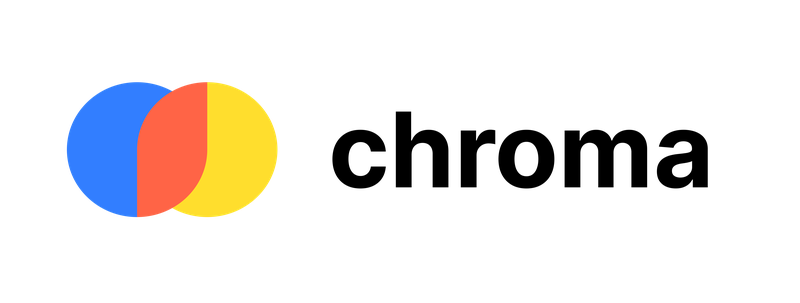
\includegraphics[width=0.8\linewidth]{images/tools/chromaDB.png}
        \caption{ChromaDB}
        \label{fig:tools_chroma}
    \end{minipage}%
    \begin{minipage}{0.3\textwidth}
        \centering
        
\includegraphics[width=0.8\linewidth]{images/tools/kafka.png}
        \caption{Kafka}
        \label{fig:tools_kafka}
    \end{minipage}%
    \begin{minipage}{0.3\textwidth}
        \centering
        
\includegraphics[width=0.8\linewidth]{images/tools/Zammad.png}
        \caption{Zammad}
        \label{fig:tools_zammad}
    \end{minipage}
\end{figure}

\section{Intégration des modèles IA}
Le projet s'appuie sur des modèles exécutés localement via \textbf{Ollama}, garantissant l'autonomie du système et la confidentialité des données.

\subsection{Modèle de langage}
Le modèle \textbf{qwen2.5:latest} est utilisé pour la validation et l'enrichissement du parsing d'incident, l'explication des causes racines, la rédaction des remédiations et la génération de texte structuré pour les rapports. En mode \texttt{MOCK\_LLM=true}, le système fonctionne de manière déterministe sans dépendance externe, ce qui facilite les tests et les démonstrations.

\subsection{Modèle d'embedding}
Le modèle \textbf{mxbai-embed-large:latest} est utilisé pour vectoriser les descriptions d'incidents et les tickets historiques. Ces vecteurs sont stockés dans Neo4j et servent à la recherche de similarité cosine.

\subsection{Provider d'embeddings}
L'interface \texttt{EmbeddingProvider} permet de changer de provider (Ollama, sentence-transformers, OpenAI, Voyage AI) sans modifier le reste du code. Cette modularité facilite les tests comparatifs et l'évolution vers d'autres modèles.

\section{Système d'agents}

\subsection{Modèle de données partagé}
L'état du graphe est matérialisé par la classe \texttt{GraphState} définie dans \texttt{shared/state.py}. Elle utilise Pydantic pour valider les données à chaque transition. Les champs principaux incluent l'incident brut, l'incident normalisé, les résultats des collecteurs, la cause racine, l'explication de remédiation, le mapping du ticket, les champs filtrés par le guardrail, le chemin du rapport, les indicateurs de notification et le journal d'audit.

\subsection{Parallélisme des collecteurs}
Les trois agents collecteurs s'exécutent en parallèle via \texttt{asyncio.gather}, avec un fallback sur \texttt{ThreadPoolExecutor} en cas de boucle déjà active. Cette approche réduit le temps total de collecte en interrogeant simultanément les logs, le CRM et le graphe Neo4j.

\subsection{Exemples d'implémentation}
L'agent d'intake utilise des expressions régulières pour extraire les identifiants métier (service, commande, client), puis détermine le type d'incident et la priorité par des règles heuristiques. Lorsque le LLM est disponible, il valide et enrichit ces extractions.

L'agent de raisonnement implémente une logique déterministe qui refuse toute hallucination : en l'absence de source suffisante, il retourne systématiquement une cause \texttt{indéterminée} avec une confiance faible.

\section{Traitement des documents}
Le traitement des documents concerne l'ingestion des données mockées dans le graphe Neo4j. Le répertoire \texttt{mocks/} contient les fichiers JSON représentant les clients, les commandes, les tickets historiques et les logs. La commande \texttt{make seed} exécute les étapes suivantes :

\begin{enumerate}
    \item Création du schéma et des contraintes Neo4j.
    \item Insertion des nœuds et des relations.
    \item Calcul et stockage des embeddings des tickets.
\end{enumerate}

\section{Génération des questions métier}
La phase d'intake transforme un incident exprimé en langage naturel en une structure métier normalisée. Le système identifie les champs essentiels (client, service, commande, type, priorité) à partir du texte brut. Cette conversion constitue la base de la génération des informations métier exploitées par les agents pour le diagnostic.

\section{Moteur de recherche}
Le moteur de recherche repose sur GraphRAG : combinaison de la recherche vectorielle native Neo4j avec un filtre de proximité de graphe. L'incident courant est vectorisé, Neo4j retourne les tickets les plus proches en similarité cosine, puis un filtre conserve ceux liés au même produit ou au même type de commande.

\section{API}
L'API est développée avec \textbf{FastAPI}. La route \texttt{/diagnose/stream} retourne un flux d'événements Server-Sent Events (SSE), chaque événement correspondant à un nœud traversé par le graphe LangGraph. Cette approche permet au client de suivre la progression du diagnostic en temps réel.

\section{Captures d'écran de l'application}
Les figures suivantes illustrent les principales interfaces de l'application.

La figure \ref{fig:streamlit_chat} montre l'interface conversationnelle Streamlit où l'opérateur saisit l'incident en langage naturel et visualise la trace des agents.

\begin{figure}[H]
    \centering
    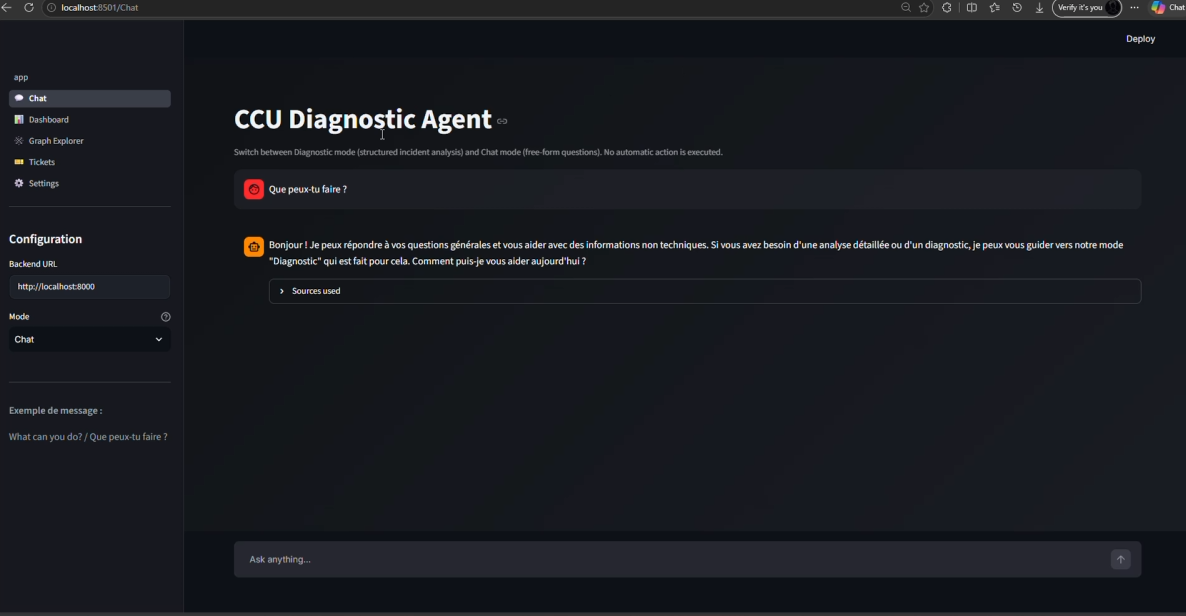
\includegraphics[width=0.9\textwidth]{images/realisation_result/Chat_agent_streamlit.png}
    \caption{Interface chatbot Streamlit}
    \label{fig:streamlit_chat}
\end{figure}

La figure \ref{fig:streamlit_dashboard} présente le tableau de bord des incidents, qui offre une vue synthétique des diagnostics en cours et passés.

\begin{figure}[H]
    \centering
    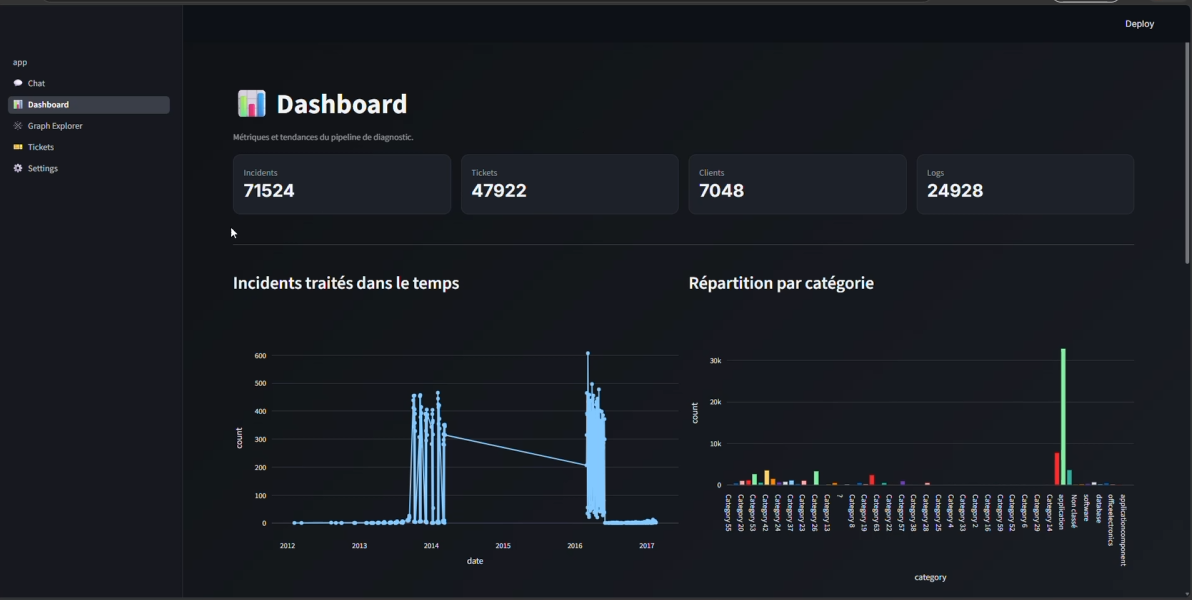
\includegraphics[width=0.9\textwidth]{images/realisation_result/dashboard_streamlit.png}
    \caption{Tableau de bord Streamlit}
    \label{fig:streamlit_dashboard}
\end{figure}

La figure \ref{fig:streamlit_tickets} affiche la liste des tickets gérés par l'application.

\begin{figure}[H]
    \centering
    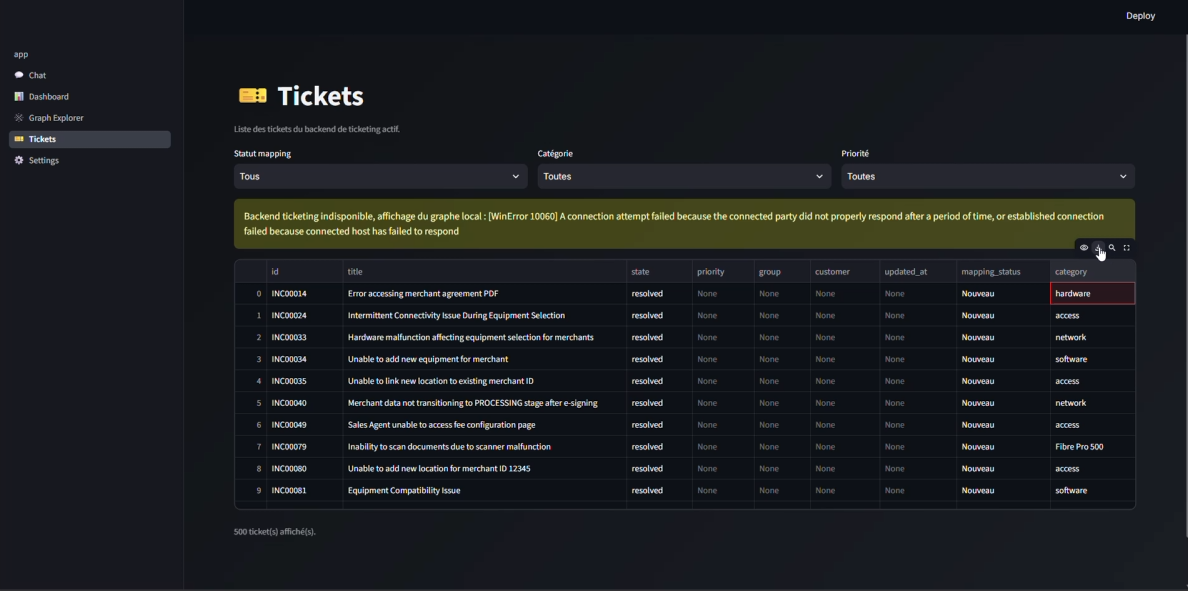
\includegraphics[width=0.9\textwidth]{images/realisation_result/liste_ticket_streamlit.png}
    \caption{Liste des tickets dans Streamlit}
    \label{fig:streamlit_tickets}
\end{figure}

La figure \ref{fig:streamlit_graph} illustre la visualisation du graphe de connaissances directement dans l'interface Streamlit.

\begin{figure}[H]
    \centering
    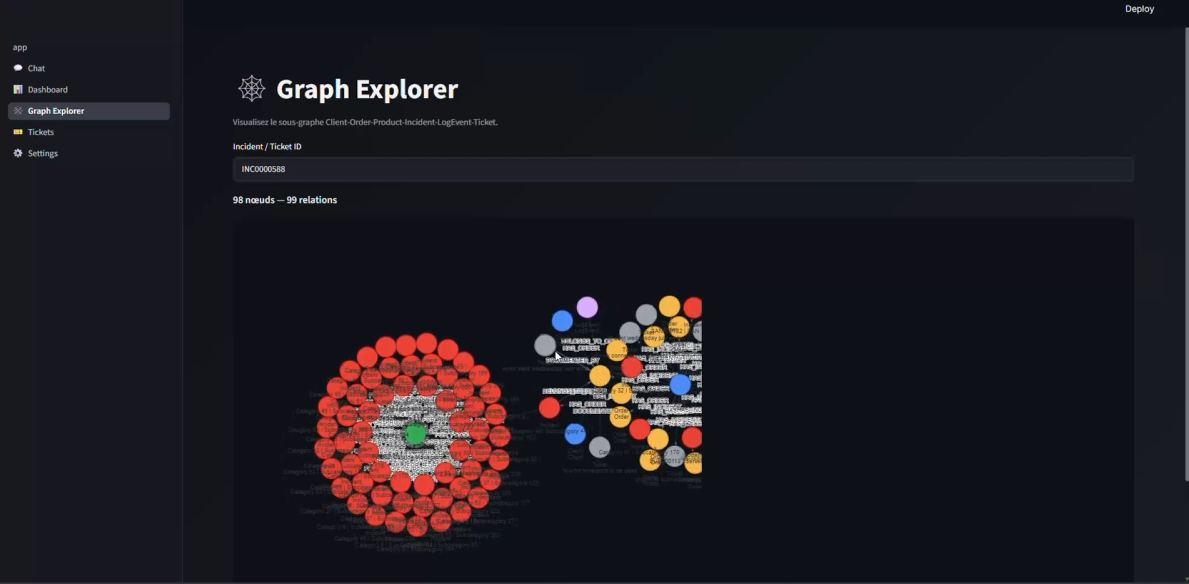
\includegraphics[width=0.9\textwidth]{images/realisation_result/Graph_streamlit.png}
    \caption{Visualisation du graphe dans Streamlit}
    \label{fig:streamlit_graph}
\end{figure}

\section*{Conclusion}
Ce chapitre a détaillé la réalisation technique du projet : environnement, stack technologique, modèles IA locaux, orchestration LangGraph, traitement des documents, moteur GraphRAG, API FastAPI et interfaces utilisateur. Le chapitre suivant présente les résultats obtenus et leur analyse.
